\documentclass[presentation]{beamer}
\usepackage{../oop-slides-pianini}
\setbeamertemplate{bibliography item}[text]
\title[OOP03 -- Interfaces]{03\\Eclipse IDE, Incapsulamento e Interfacce}
\author[Pianini]{Danilo Pianini\\Giovanni Ciatto, Angelo Croatti, Mirko Viroli}

\begin{document}
	
\frame[label=coverpage]{\titlepage}

\begin{frame}<beamer>
	\frametitle{Outline}
	\tableofcontents[]
\end{frame}

\section{Eclipse IDE}
\subsection{Introduzione}

\begin{frame}{Integrated Development Environment (IDE)}
	\begin{block}{}
		\emph{A software suite that consolidates the basic tools developers need to write and test software. An IDE contains a code editor, a compiler and a debugger that the developer accesses through a single user interface.}
	\end{block}
	\begin{itemize}
		\item Ambiente integrato per la creazione e la gestione di progetti software.
		\begin{itemize}
			\item Un progetto, per un IDE, è composto da una collezione organizzata di risorse: sorgenti, librerie, compilati, documentazione, \dots
		\end{itemize}
		\item Componenti tipici di un IDE:
		\begin{itemize}
			\item Editor di testo con syntax highlighting (e code completion)
			\item Compilatore
			\item Macchina(e) virtuale per l'esecuzione e il debugging delle applicazioni
			\item Strumenti per agevolare il deployment (distribuzione) delle applicazioni
		\end{itemize}
		\item Esempi di IDE:
		\begin{itemize}
			\item Eclipse, NetBeans, IntelliJ IDEA, Microsoft Visual Studio, XCode, \dots
		\end{itemize}
	\end{itemize}
\end{frame}

\begin{frame}{Diffusione dei principali IDE}
	\begin{center}
		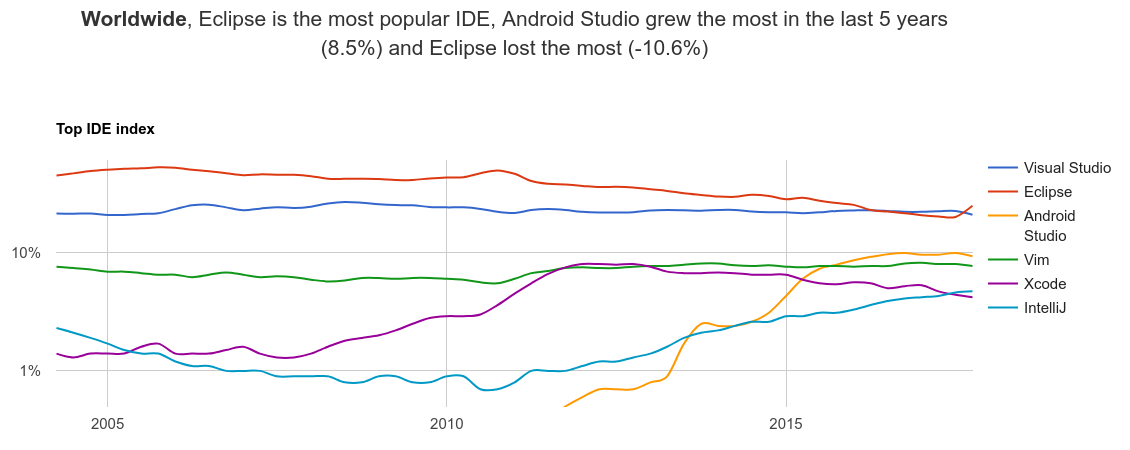
\includegraphics[width=\textwidth]{img/ide2017world.png}
	\end{center}
\end{frame}



\fr{Eclipse Overview}{
	\bl{Overview}{
		\iz{
			\item Eclipse è un IDE open-source scritto in Java 
			\item Disponibile per diverse piattaforme (Windows, Linux, Mac OSX, ..)
			\item 	.. e sotto forma di diverse distribuzioni 
				\iz{
					\item	Standard, per sviluppatori J2EE/C/C++/Python/Web.. 
				}
			}
	}
	\bl{Un po' di storia}{
		\iz{
			\item Nato nei laboratori di ricerca IBM (alphaWorks) 
			\item	Successivamente	donato alla comunità open-source che ora ne cura lo sviluppo per mezzo di un'apposita fondazione
			\item Correntemente supportato/utilizzato da un vasto numero di sviluppatori, sia in ambito accademico che industriale
		}
	}
}

\begin{frame}[allowframebreaks]{Astrazioni di base}
	\begin{block}{Workspace}
		Directory dove Eclipse salva e carica le impostazioni di un certo numero di progetti. Tipicamente contiene anche i progetti (che possono però anche essere importati da altre directory)
	\end{block}
	\begin{block}{Progetto}
		Directory contenente una collezione di risorse opportunamente organizzate, tipicamente rappresentanti un software o una parte di un software
	\end{block}
	\begin{block}{Plug-in}
		Software installabile opzionalmente che estende le capacità dell'IDE, ad esempio:
		\begin{itemize}
			\item controllare la qualità del codice Java;
			\item aggiungere supporto ad ulteriori linguaggi;
			\item usare sistemi di build diversi da quello predefinito (Gradle, Maven...);
		\end{itemize}
	\end{block}
	\begin{block}{View}
		Componente dell'interfaccia di Eclipse.
		\begin{itemize}
			\item Tipicamente numerose view sono aperte contemporaneamente;
			\item Ciascuna offre una micro-funzionalità, ad esempio:
			\begin{itemize}
				\item Package Explorer --- fornisce una vista dei progetti e della loro struttura;
				\item Console --- consente di usare un terminale interno all'IDE invece del terminale di sistema;
				\item Outline --- mostra un riassunto dei componenti della classe attualmente aperta, elencando i membri, consentendo di filtrarli (ad esempio, nascondendo i privati) e di ordinarli (ad esempio in ordine alfabetico);
				\item Problems --- elenca gli eventuali problemi che affliggono il progetto (errori di configurazione, sorgenti che non compilano, warnings...)
				\item 
			\end{itemize}
		\end{itemize}
	\end{block}
	\begin{block}{Perspective}
		Insieme di view che vengono. Cambiare perspective consente di cambiare rapidamente le view attive. Tipicamente, si usano perspective diverse per fasi diverse dello sviluppo. Ne vedremo sicuramente due:
		\begin{itemize}
			\item Java --- per lo sviluppo di applicazioni Java
			\item Debug --- per il debug di applicazioni (prossima lezione!)
		\end{itemize}
	\end{block}
\end{frame}


\subsection{Avvio e creazione di progetti}

\fr{Avvio di Eclipse: Scelta del Workspace}{
	\fg{width=\textwidth}{img/eclipse_startup.png}	
}
\fr{Creazione di Progetti Java 1/3}{
	\fg{height=0.85\textheight}{img/new_prj1.png}
}

\fr{Creazione di Progetti Java 2/3}{
	\fg{height=0.85\textheight}{img/new_prj2.png}
}

\fr{Creazione di Progetti Java 3/3}{
	\fg{height=0.85\textheight}{img/new_prj3.png}
}

\fr{Compilazione dei Sorgenti}{
	\fg{height=0.3\textheight}{img/eclipse_build.png}
	\bl{Due diverse possibilità}{
		\iz{
			\item Compilazione automatica
			\iz{
				\item Il compilatore viene invocato automaticamente dall'IDE ad ogni modifica (salvata) ai sorgenti del progetto
			}
			\item Compilazione manuale
			\iz{
				\item Attiva quando è disabilitata la compilazione automatica
				\item Il compilatore viene invocato a seguito di un esplicito click dello sviluppatore su \textit{``Build All''}
			}
		}
	}
}

\fr{Creazione di un Package 1/2}{
	\fg{height=0.8\textheight}{img/new_package1.png}
}

\fr{Creazione di un Package 2/2}{
	\fg{height=0.8\textheight}{img/new_package2.png}
}

\fr{Creazione di una Classe 1/2}{
	\fg{height=0.8\textheight}{img/new_class1.png}
}

\fr{Creazione di una Classe 2/2}{
	\fg{height=0.8\textheight}{img/new_class2.png}
}

\fr{JDT: Code Completion e Syntax Highlighting}{
	\fg{height=0.8\textheight}{img/sh_cc.png}
}

\fr{Esecuzione di Applicazioni}{
	\fg{height=0.8\textheight}{img/run1.png}
}

\fr{Esecuzione di Applicazioni: Un Alternativa 1/2}{
	\fg{height=0.8\textheight}{img/run2.png}
}

\fr{Esecuzione di Applicazioni: Un Alternativa 2/2}{
	\fg{height=0.8\textheight}{img/run3.png}
}

\fr{Esecuzione di Applicazioni: Output}{
	\fg{height=0.8\textheight}{img/run4.png}
}

\fr{Importazione di Progetti 1/2}{
	\fg{height=0.8\textheight}{img/import_prj1.png}
}

\fr{Importazione di Progetti Esistenti 2/2}{
	\fg{height=0.8\textheight}{img/import_prj2.png}
}

\subsection{Eclipse: Maggiori Dettagli}

\fr{Eclipse Architecture}{
	
	\bl{Eclipse ha una architettura organizzata a plug-in}{
		\iz{
			\item Un plug-in è un modulo (classi + meta-informazioni + manifest file) auto-contenuto che incapsula una certa funzionalità
				\iz{
						\item File editor specifici, wizard, build, compilazione e debugging di sorgenti
						\item Costituisce l'unità funzionale elementare dell'architettura
				}
			\item Possono essere definite relazioni di dipendenza, composizione, etc. specifiche dell'astrazione plug-in (non parte dell'OOP)
				\iz{
					\item Non le tratteremo nel dettaglio in questo corso
				}
		}
	}
	
	\bl{Eclipse come IDE Modulare}{
		\iz{
			\item Nuovi plug-in possono essere liberamente installati al bisogno
				\iz{
					\item Ne esistono moltissimi open-source, altri sviluppati da aziende e università
				}
			\item Supporto nativo lo sviluppo di nuovi plug-in
				\iz{
					\item Plug-in Development Environment (PDE)
				}
		}
	}
}


\fr{Plug-in and Perspective}{

	\bl{Che relazione tra plug-in e perspective?}{
		\iz{
			\item Le prospettive disponibili sono definite dai plug-in installati
			\item Prospettive disponibili di default (e.g. Resource, Java, Debug, Git,..)
		}
	}
	\bl{Descrizione di alcune delle perspective di default}{
		\iz{
			\item \textcolor{blue}{Resource perspective}: permette di navigare e interagire con le risorse in termini di file
				\iz{
					\item  Il progetto è visto come una collezione di file e directory, che è possibile creare, modificare, spostare, etc.
				}
		
			\item \textcolor{blue}{Java perspective}: fornisce viste ed editor per gestire tutte le attività più significative per lo sviluppo di progetti Java
				\iz{
					\item Realizzata da un insieme di plug-in che prendono il nome di JDT (Java Development Tools)
				}

			\item ...
			
		}
	}
}

\fr{Resource Perspective (Default Perspective)}{
		\fg{height=0.85\textheight}{img/default_perspective.png}
}

\fr{JDT e Java Perspective}{
		\fg{height=0.85\textheight}{img/jdt_perspective.png}
}

\section{Lab Startup}

\fr{Preparazione Ambiente di Lavoro 1/2}{
\iz{
\item Accendere il PC
\item Loggarsi sul sito del corso
\iz{
\item\textcolor{blue}{\url{https://bit.ly/oop2017cesena}}
}
\item Scaricare dalla sezione \texttt{lab} del sito il file \texttt{lab03.zip} contenente il materiale dell'esercitazione odierna
\item Spostare il file scaricato sul Desktop
\item Decomprimere il file usando 7zip (o un programma analogo) sul Desktop
}
}

\fr{Preparazione Ambiente di Lavoro 2/2}{
	\iz{
		\item Copiare la cartella scompattata all'interno del workspace di Eclipse
		\item Importare il progetto \texttt{lab03} con la procedura di importazione dei progetti mostrata nelle slide precedenti
		\item Al termine della procedura l'ambiente di lavoro sarà circa come segue
	}
	\fg{height=0.3\textheight}{img/prj_importato.png}
	
}


\fr{Modalità di Lavoro}{
	\bl{}{
		\en{
			\item Leggere la consegna
			\item Risolvere l'esercizio in autonomia
			\item Cercare di risolvere autonomamente eventuali piccoli problemi che possono verificarsi durante lo svolgimento degli esercizi
			\item \alert{Utilizzare le funzioni di test presenti nei sorgenti per il testing dell'esercizio}
			\item Contattare i docenti nel caso vi troviate a lungo bloccati nella risoluzione di uno specifico esercizio
			\item A esercizio ultimato contattare i docenti per un rapido controllo della soluzione realizzata
			\item Proseguire con l'esercizio seguente
		}
	}
}


\section{Warm up: miglioramento di classi già implementate}

\fr{Applichiamo il Principio di Incapsulamento 1/2}{
	\bl{Analizzare la classe \cil{oop.lab03.encapsulation.Student}}{
		\iz{
			\item E' una versione modificata della classe definita nel package \cil{oop.lab02.constructors} e vista la settimana scorsa
			\item Confrontare la classe con la sua versione precedente
			\item Dettaglio delle modifiche apportate
				\en{
					\item I campi della classe ora sono tutti privati
					\iz{
						\item Non c'è necessità di renderli direttamente accessibili: \alert{così il cliente di una classe non è mai influenzato da possibile modifiche future riguardanti meri aspetti realizzativi}
					}
					\item Introduzione di selettori per leggere le informazioni di stato
					\iz{
						\item \cil{getName, getSurname,}..
					}
				}
		}
	}
}

\fr{Applichiamo il Principio di Incapsulamento 2/2}{
	\bl{}{
		Modificare le classi Calculator e Smartphone contenute nel package \cil{oop.lab03.encapsulation} applicando il principio di incapsulamento
	}
	
	\bl{Passi da seguire}{
		\en{
			\item Rendere privati tutti i campi delle classi
			\item Introdurre degli opportuni selettori per recuperare le informazioni di stato (campi) di interesse
		}
	}
}

\section{Esercizi base}

\fr{\cil{oop.lab03.encapsulation.AccountHolder}}{
	\bl{}{
		\iz{
			\item Analizzare la classe \cil{AccountHolder}
			\item Modella un generico utilizzatore di un conto bancario, identificato dal campo \cil{userID} (di tipo \cil{int}) della classe
			\item E' stata realizzata applicando il principio di incapsulamento
				\iz{
					\item Cosa che dovremo fare da ora (\textit{sempre, in automatico}) per \alert{tutte} le classi che costruiremo
			}
		}
	}
	\bl{}{
		Implementare il metodo \cil{String toString()} lasciato incompleto
			\iz{
				\item Metodo utilizzato convenzionalmente dalle librerie Java e dall'operatore di concatenazione \texttt{+} tra stringhe, al fine di restituire la rappresentazione testuale di un oggetto
			}
	}
}
	

\fr{\cil{oop.lab03.encapsulation.SimpleBankAccount} 1/2}{
	\bl{Modella un generico conto bancario di un AccountHolder}{
		Completare la classe seguendo le istruzioni riportate nelle slide e nei commenti della classe stessa
	}

	\bl{Campi}{
		\iz{
		  \item \cil{double balance // Ammontare conto} 
		  \item \cil{int usrID // Id AccountHolder}
		  \item \cil{int nTransactions // N. prelievi/depositi}
		  \item \cil{double ATM_TRANSACTION_FEE = 1 // Costante relativa al costo aggiuntivo delle operazioni via ATM}
		}
	}
	
	\bl{Costruttori}{
		\iz{
			\item \cil{public SimpleBankAccount(int usrID, double initAmount)}
		}
	}
}

\fr{\cil{oop.lab03.encapsulation.SimpleBankAccount} 2/2}{
	
	\bl{Metodi}{
		\iz{
			\item Selettori, uno per campo (da implementare da zero)
			\item \cil{public void deposit(int usrID, double amount)}
			\item \cil{public void withdraw(int usrID, double amount)}
			\item \cil{public void depositFromATM(int usrID, double amount)}
			\item \cil{public void withdrawFromATM(int usrID, double amount)}
			\item \cil{private boolean checkUser(int id) //Già implementato}
		}
	}
	
	\bl{Nota}{
		Fare riferimento al sorgente della classe per capire in dettaglio come implementare i vari metodi
	}
}


\fr{Test di SimpleBankAccount}{
	\bl{}{
		Effettuare il test della classe \cil{SimpleBankAccount} appena implementata seguendo le indicazioni fornite nei commenti in \cil{oop.lab03.encapsulation.TestSimpleBankAccount} 
	}
}

\begin{frame}[allowframebreaks]{\texttt{oop.lab03.interfaces.BankAccount}}
	\bl{}{
		Modificare la classe \cil{SimpleBankAccount} in modo da implementare l'interfaccia \cil{BankAccount}
                \iz{ \item realizzare solamente i metodi necessari alla corretta implementazione dell'interfaccia da parte di \cil{SimpleBankAccount}}
	}
	\bl{\cil{oop.lab03.interfaces.BankAccount}}{
		\sizedcode{\scriptsize}{../../workspace/lab03/src/oop/lab03/interfaces/BankAccount.java}
	}
	\bl{Requisiti per implementare il metodo \cil{void computeManagementFees(int usrID)}}{
		\en{
			\item Il metodo, quando invocato, dovrà detrarre dal conto le \emph{spese di gestione} previste dalla banca  
			\item In prima battuta modellare le \emph{spese di gestione} come \textbf{double} di valore pari a \textbf{5 Euro}
				\iz{
					\item Ricordate quanto detto durante lo scorso laboratorio a proposito di \emph{magic number} e utilizzo delle \emph{costanti}?
				}
		}
	}
\end{frame}

\fr{\cil{oop.lab03.interfaces.StrictBankAccount}}{	
	\bl{}{Implementare in autonomia la classe \cil{StrictBankAccount}}
	\bl{Linee guida}{
		\iz{
			\item La classe dovrà implementare l'interfaccia \cil{BankAccount}
			\item Al solito, le operazioni sul conto dovranno essere abilitate solo se lo user id corrisponde a quello a cui il conto è stato associato
			\item Non dovrà essere possibile effettuare dei prelievi se l'ammontare da prelevare specificato è superiore alla disponibilità corrente del conto
				\iz{
					\item Le operazioni di prelievo in questo caso non dovranno fare nulla
				}
			\item Le spese di gestione dovranno essere calcolate come segue
				\iz{
					\item Costo fisso (\emph{5 Euro} come nel caso precedente) \alert{più}
					\item Costo variabile in base al numero di transazioni effettuate (costo di ogni singola transazione \emph{0.1 Euro})
				}
		}
	}	
}
	
\fr{\cil{SimpleBankAccount e StrictBankAccount: Test}}{	
		\bl{}{
			Effettuare il test delle classi \cil{SimpleBankAccount} e \cil{StrictBankAccount} appena implementate seguendo le indicazioni fornite nei commenti in \cil{oop.lab03.interfaces.TestBankAccount} 
		}
}

\section{ACME-Exams}

\fr{ACME-Exams: Sistema SW per Gestire Appelli Universitari}{
	\bl{Requisiti}{
		\iz{
			\item Target di utenza: studenti e docenti
			\item Gli studenti possono: vedere gli esami esistenti, registrarsi, visualizzare i voti di esami conclusi, visualizzare statistiche relative ai loro esami
			\item I docenti possono: creare nuovi appelli, inserire voti per esami passati, visualizzare statistiche relative agli appelli
		}
	}	
}

\fr{Modelliamo gli Utenti: Interfaccia User}{
	\bl{}{
		\iz{
			\item \cil{IUser} definisce l'interfaccia di un generico utente di ACME-Exams
			\item Analizzare l'interfaccia \cil{User} e la classe \cil{Student} che la implementa
		}
	}
	\bl{\cil{oop.lab03.acme.User}}{
		\sizedcode{\scriptsize}{../../workspace/lab03/src/oop/lab03/acme/User.java}
	}
}

\fr{\cil{oop.lab03.acme.Professor}}{
	\bl{Implementare la classe \cil{Professor} (dovrà implementare \cil{User})}{
		Modella un generico docente
		\iz{
			\item Campi
			\iz{
				\item \cil{int id; String name, surname, password}
				\item \cil{String[] courses} (nome dei corsi tenuti)
			}
			\item Un solo costruttore
			\iz{
				\item Specifica l'insieme di parametri necessario ad inizializzare tutti i campi della classe \cil{Professor} meno lo \cil{username} (da ricavare come è stato fatto nella classe \cil{Student})
			}
			\item Selettori
			\iz{
				\item Uno per campo (p.e. \cil{public int getId()})
			}
			\item Modificatori
			\iz{
				\item \cil{public void replaceCourse(String course, int idx)}
				\iz{
					\item Sostituisce il corso all'indice \cil{idx} con quello fornito in input
				}
				\item \cil{public void replaceAllCourses(String[] courses)}
				\iz{
					\item Sostituisce tutti i corsi tenuti dal docente
				}
			}
		}
	}
}

\begin{frame}[allowframebreaks]{Composizione}
	\bl{Implementare la classe \cil{oop.lab03.acme.Exam}}{
		Modella un generico appello d'esame all'interno di ACME-Exams
		\iz{
			\item Campi
			\iz{
				\item \cil{int id, nMaxStudents, nRegisteredStudents;}
				\item \cil{String courseName;}
				\item \cil{Student[] students; Professor professor}
				\item \cil{ExamRoom room} (classe che modella un aula, \textcolor{blue}{fornita tra i sorgenti})
			}
			\item Un solo costruttore
			\iz{
				\item Specifica i parametri necessari ad inizializzare tutti i campi tranne \cil{nRegisteredStudent} (da inizializzare a zero) e \cil{students}
			}
			\item Metodi
			\iz{
				\item Un selettore per campo (p.e. \cil{public int getId()})
				\item \cil{public void registerStudent(Student student)}
				\iz{
					\item Iscrive lo studente all'appello. Qualora si sia raggiunto il limite massimo di studenti per l'appello non fa nulla.
				}
			}
		}
	}
	\bl{Altri Metodi}{
		\iz{
			\item \cil{String toString()}
				\iz{
					\item Solito metodo che fornisce una rappresentazione in stringa
					\item Appoggiarsi ad \cil{Arrays.toString(<tipo> array)} per ottenere una rappresentazione in formato stringa di un array
				}
		}
	}

	\bl{Note}{
		\iz{
			\item Creare l'array di studenti nel costruttore fissandone la dimensione a \cil{nMaxStudents}
			\item Utilizzare la variabile \cil{nRegisteredStudents}
				\iz{
					\item Per tenere traccia del numero di studenti correntemente registrati
					\item Come indice in cui salvare il prossimo studente da iscrivere (metodo \cil{registerStudent})
				}
		}
	}
\end{frame}

\fr{\cil{oop.lab03.acme.Testing}}{
	\bl{}{
		Seguire le linee guida riportate nella classe \cil{Testing} per effettuare il testing delle classi \cil{Professor} e \cil{Exam}
	}
}
\section{Esercizi Avanzati}

\fr{Shape: un'interfaccia per modellare figure geometriche}{
        \bl{\cil{oop.lab03.interfaces.Shape.java}}{Realizzare \textbf{da zero} un'interfaccia che consenta di calcolare \textbf{area} e \textbf{perimetro} di una qualsivoglia \textbf{figura geometrica}}
	\bl{Metodi da definire sull'interfaccia}{
		\iz{	
			\item \cil{double getArea ()}
			\item \cil{double getPerimeter ()}
		}	
	}
}

\fr{\cil{oop.lab03.shapes.Circle}}{
	\bx{Realizzare da zero la classe \cil{Circle} che, implementando l'interfaccia \cil{Shape}, consenta di definire un cerchio
		\iz{	
			\item Fate attenzione alla definizione dei campi necessari e del costruttore della classe
		}
	}
	
}
	
\fr{Estensione per Figure con Lati Limitati}{

	\bl{Realizzare \cil{oop.lab03.interfaces.Polygon} che estende \cil{Shape}}{
		\iz{
			\item definire il metodo \cil{int getNumEdges()} che restituisce il numero di lati della forma geometrica
			\item I metodi definiti in \cil{Shape} vengono perciò \textit{ereditati}
			\item Pertanto, le classi che implementeranno \cil{Polygon} dovranno obbligatoriamente definire 3 metodi relativi a questa interfaccia
		}
	}	
}

\fr{Square, Rectangle and Triangle}{
	\bl{Implementare le classi \cil{Square}, \cil{Rectangle} e \cil{Triangle}}{
		\iz{
			\item Le tre classi dovranno implementare \cil{Polygon}
			\item Implementare opportunamente i metodi dell'interfaccia
		}
	}
	
	\bl{}{
		Per semplicità, per la classe \cil{Triangle} implementare un costruttore che richiede in input anche l'altezza relativa ad uno dei tre lati (sarà banale in questo modo calcolare l'area)
	}
}

\fr{WorkWithShapes}{
	\bl{}{
		Una volta terminata l'implementazione delle varie classi, implementare in \cil{WorkWithShapes} un insieme di test a piacere stampando in stdout il risultato del calcolo di area/perimetro per diverse figure geometriche
	}
}

%\begin{frame}[allowframebreaks]
% \frametitle{Bibliography}
%	\bibliographystyle{plain}
%	\small
% \bibliography{biblio}
%\end{frame}


\end{document}



%%%%%%%%%%ECLIPSE GOING TO LAB 04

